% !TeX root = RJwrapper.tex
\title{A clustering algorithm to organize satellite hotspots data for
the purpose of tracking bushfires remotely}
\author{by Weihao Li, Emily Dodwell, and Dianne Cook}

\maketitle

\abstract{%
An abstract of less than 150 words.
}

\hypertarget{introduction}{%
\subsection{Introduction}\label{introduction}}

Bushfires are a major problem for Australia, and many other parts of the
globe. There is concern that as the climate becomes hotter, and drier,
that the impact of fires becomes much more severe and extensive. In
Australia, the 2019-2020 fires were the worst on record causing
extensive ecological damage, as well as damage to agricultural
resources, properties and infrastructure. The Wollemi pine, rare
prehistoric trees, required special forces intervention to prevent the
last stands in the world, in remote wilderness areas, from being turned
into ash.

Contributing to the problem is that many fires started in very remote
areas, locations deep into the temperate forests ignited by lightning,
that are virtually impossible to access or to monitor. Satellite data
provides a possible solution to this, particularly remotely sensed
hotspot data, which may be useful in detecting new ignitions and
movements of fires. Understanding fires in remote areas using satellite
data may provide some help in developing effective strategies for
mitigating bushfire impact.

This work addresses this topic. Using hotspot data, can we cluster in
space and time, in order to determine (1) points of ignition and (2)
track the movement of bushfires. The algorithm is implemented in the R
package \CRANpkg{spotoroo}.

This paper is organised as follows. The next section provides an
introduction to the literature on spatiotemporal clustering and bushfire
modeling and dynamics. Section \protect\hyperlink{algorithm}{Algorithm}
describes the clustering algorithm, and section
\protect\hyperlink{application}{Application} illustrates how the
resulting data can be used to study bushfire ignition.

\hypertarget{background}{%
\subsection{Background}\label{background}}

literature review

\hypertarget{algorithm}{%
\subsection{Algorithm}\label{algorithm}}

\hypertarget{data-source}{%
\subsubsection{Data source}\label{data-source}}

The illustration of this algorithm will use the wild fire product
(produced from Himawari-8) supplied by the P-Tree System, Japan
Aerospace Exploration Agency (JAXA) \citeyearpar{jaxa} as the data
source. This wild fire product will be referred as the hotspot data in
this paper. It contains records of 1989572 hotspots from October 2019 to
March 2020 in the full disk of 140 \textdegree east longitude with 0.02
\textdegree spatial resolution and 10 minutes temporal resolution.

The data pre-processing procedure includes selecting hotspots within the
boundary of Victoria and filtering hotspots with a threshold (irradiance
over 100 watts per square metre) suggested by landscape ecologist and
spatial scientist Dr.~Grant Williamson \citeyearpar{hotspots} to reduce
noise from the background.

The final hotspot dataset contains 75936 observations with ID,
longitude, latitude and observed date as fields. The overall
distribution of these hotspots is shown in Figure \ref{fig:hotspots}.

\begin{Schunk}
\begin{figure}

{\centering 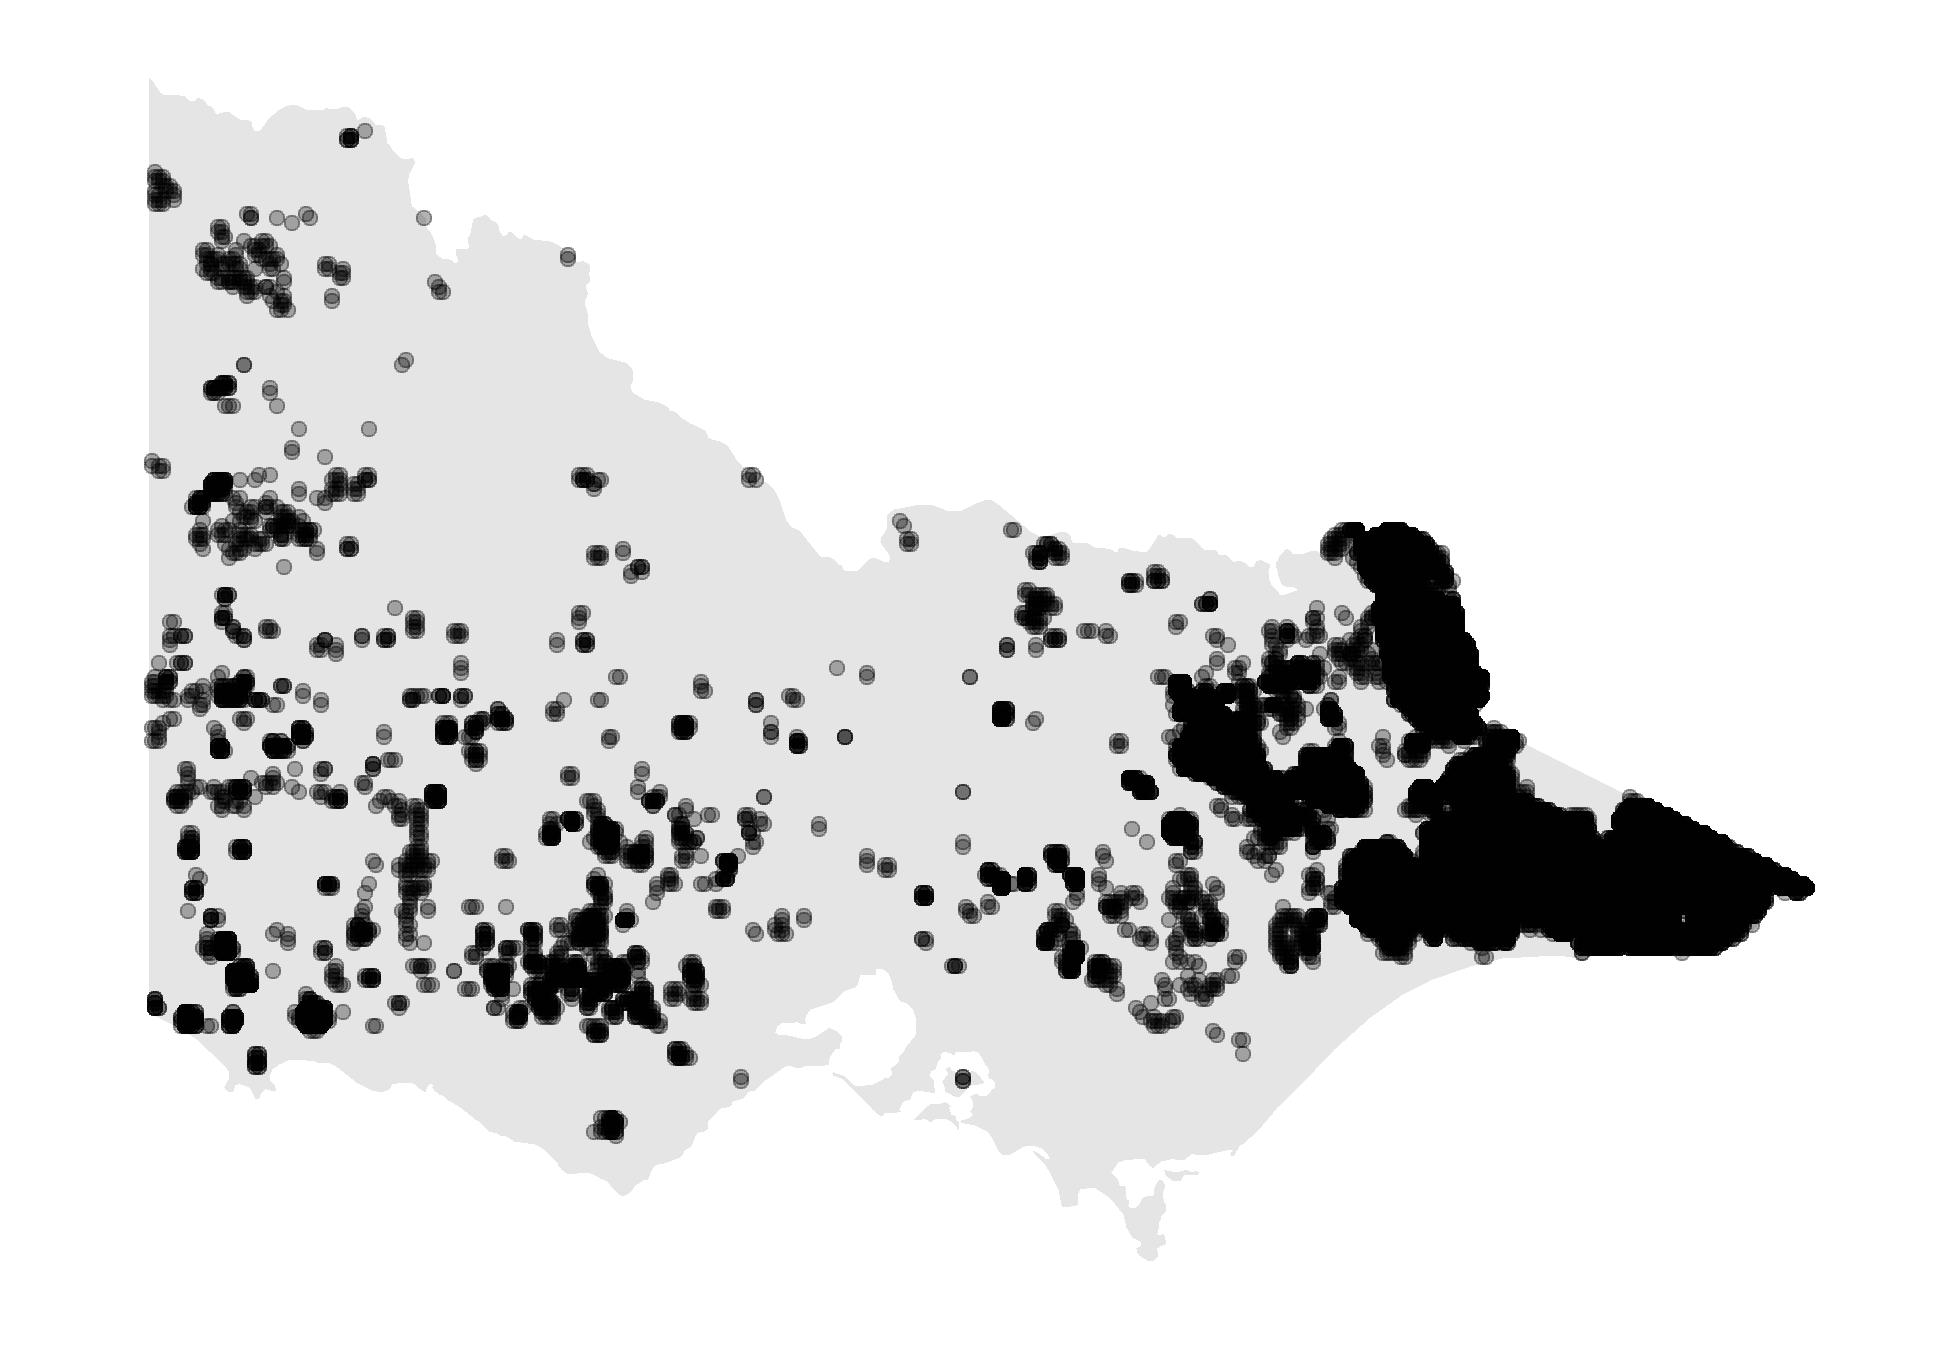
\includegraphics[width=0.8\linewidth]{figures/before_clustering} 

}

\caption[The distribution of hotspots in Victoria during 2019-2020 Australia bushfire season]{The distribution of hotspots in Victoria during 2019-2020 Australia bushfire season.}\label{fig:hotspots}
\end{figure}
\end{Schunk}

\hypertarget{steps}{%
\subsubsection{Steps}\label{steps}}

The spatiotemporal clustering algorithm is consist of 3 steps, (1)
divide hotspots into intervals, (2) cluster hotspots spatially, and (3)
update the memberships. These three steps will be described in details
in the rest of the section.

\textbf{1. Divide hotspots into intervals}

Despite hotspot data can be clustered using ordinary algorithms, like
K-means, in the three-dimensional Euclidean space, the clustering
results could be highly sensitive to the scaling of the temporal
dimension \citep{kisilevich2009spatio}. Besides, one of the
characteristics of the hotspot data is cloud cover could lead to missing
observations of a bushfire in several hours. This suggests that hotspots
with long intervals may present connections. One possible solution to
these two issues is to divide hotspot data into intervals then perform
clustering spatially only, such that the temporal dependence between
hotspots could be predetermined by a parameter \(ActiveTime\). The
interpretation of \(ActiveTime\) is the time a fire can stay smouldering
but undetectable by satellite before flaring up again.

Given a certain value of \(ActiveTime\) and an integer length of the
time frame \(T\), the algorithm will define several intervals,

\[\boldsymbol{S}_t = [max(1,t-ActiveTime),t],~~t = 1,2,...,T\],

where both \(T\) and \(t\) have the same unit as \(ActiveTime\).

For example, if the dataset contains 48 hours of hotspot data and the
\(ACtiveTime = 24~hours\), there will be 48 intervals defined by the
algorithm, \(\boldsymbol{S}_1,\boldsymbol{S}_2,..,\boldsymbol{S}_{48}\),
where

\begin{align*}
\boldsymbol{S}_1 &= [1,1]\\
\boldsymbol{S}_2 &= [1,2]\\
&...\\
\boldsymbol{S}_{25} &= [1,25]\\
\boldsymbol{S}_{26} &= [2,26]\\
&...\\
\boldsymbol{S}_{47} &= [23,47]\\
\boldsymbol{S}_{48} &= [24,48]
\end{align*}

\textbf{2. Cluster hotspots spatially}

The previous step breaks the temporal dimension. Hence, the following
step only needs to address the hotspots spatially by introducing another
parameter \(AdjDist\). \(AdjDist\) represents the potential distance a
fire can spread with respect to the temporal resolution of the data. For
example, let \(AdjDist = 3000 m\) and the temporal resolution of the
data is 10-minute, then the potential speed of the bushfire is
\(3000m/10~min = 18km/h\).

Given a fixed value of \(AdjDist\) and the interval
\(\boldsymbol{S}_t\), the algorithm will:

\begin{enumerate}
\def\labelenumi{(\alph{enumi})}
\item
  Append a randomly selected hotspot \(h_i\) to a empty list
  \(\boldsymbol{L}\), where \(h_i\) is the \(i\)th hotspot in the
  interval \(\boldsymbol{S}_t\), and let pointer \(\boldsymbol{P}\)
  points to the first element of the list \(\boldsymbol{L}\).
\item
  Visit every \(h_i\) where \(h_i \notin \boldsymbol{L}\). If
  \(geodesic(h_i, \boldsymbol{P})\leq AdjDist\), append \(h_i\) to list
  \(\boldsymbol{L}\).
\item
  Move pointer \(\boldsymbol{P}\) to the next item of the list
  \(\boldsymbol{L}\).
\item
  Repeat (b) and (c) till the pointer \(\boldsymbol{P}\) reaches to the
  end of the list \(\boldsymbol{L}\).
\item
  For all hotspots \(h_i \in \boldsymbol{L}\), assign a new membership
  to them. Pop these hotspots from the interval \(\boldsymbol{S}_t\).
  Repeat (a) to (e) if interval \(\boldsymbol{S}_t\) is not empty.
\item
  Recover the interval \(\boldsymbol{S}_t\) and record the memberships.
\end{enumerate}

Figure \ref{fig:step2figs} gives an concise example of this step.

\begin{Schunk}
\begin{figure}

{\centering 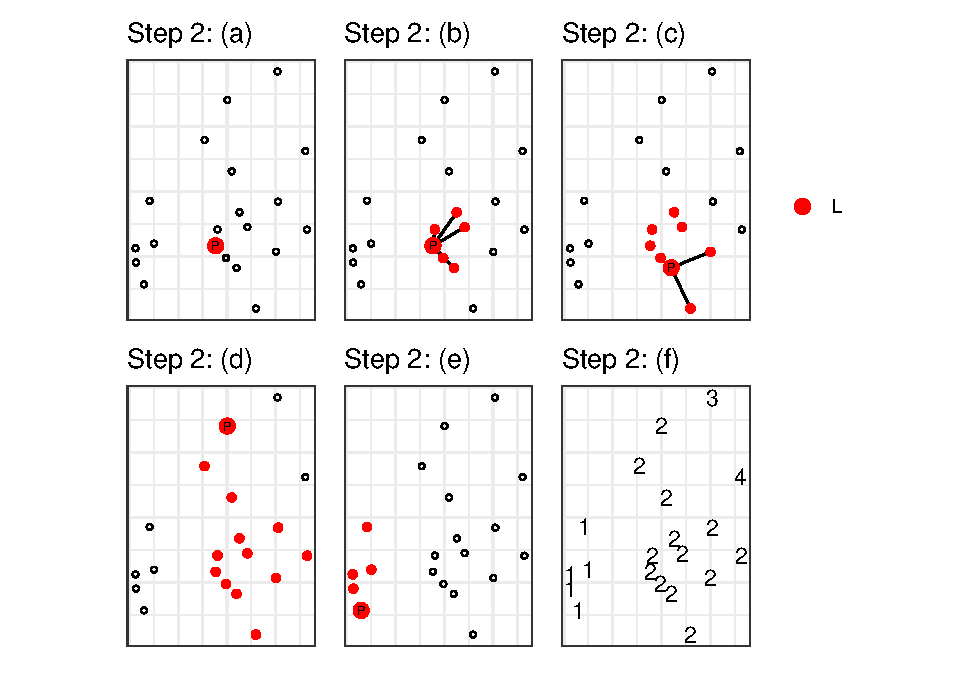
\includegraphics[width=0.8\linewidth]{clustering_paper_files/figure-latex/step2figs-1} 

}

\caption{An example of step 2 given 20 hotspots in interval $\boldsymbol{S}_t$. (a) A hotspot is selected randomly as the first item of list $\boldsymbol{L}$ and the pointer $\boldsymbol{P}$. Hotspots in list $\boldsymbol{L}$ are in red. Pointer $\boldsymbol{P}$ is drawn with larger marker size. (b) Nearby hotspots of the pointer $\boldsymbol{P}$ are appended to the list $\boldsymbol{L}$. (c) Move pointer $\boldsymbol{P}$ to the next item of list $\boldsymbol{L}$ and append the nearby hotspots to list $\boldsymbol{L}$. (d) The first cluster is identified via repeating substep (c). (e) Clear the list $\boldsymbol{L}$, then randomly select an unassigned hotspot to identify another cluster. (f) The final clustering result is produced via repeating substep (d). The labels show the cluster each hotspot belongs to.}\label{fig:step2figs}
\end{figure}
\end{Schunk}

\textbf{3. Update the memberships}

With clustering results for each interval, the next step is to update
the memberships by bringing in information from earlier intervals.

This step starts from \(t=2\) till \(t=T\). Given the interval
\(\boldsymbol{S}_t\), the algorithm will,

\begin{enumerate}
\def\labelenumi{(\alph{enumi})}
\item
  Let \(h_i\) succeeds its membership from \(\boldsymbol{S}_{t-1}\), if
  \(h_i\) belongs to \(\boldsymbol{S}_{t-1}\), where \(h_i\) is the
  \(i\)th hotspot in the interval \(\boldsymbol{S}_t\). These hotspots
  are collected by a set \(\boldsymbol{H}_s = \{h_s^1,h_s^2,...\}\).
\item
  Set \(\boldsymbol{H}_c = \{h_c^1,h_c^2,...\}\), where \(h_c^i\) is the
  \(i\)th hotspot in set \(\boldsymbol{H}_c\). \(h_c^i\) belongs to
  \(\boldsymbol{S}_t\) but does not belong to \(\boldsymbol{S}_{t-1}\).
  If \(h_c^i\) being clustered into the same component with \(h_s^j\) in
  interval \(\boldsymbol{S}_t\), \(h_c^i\) succeeds the membership from
  the nearest \(h_s^j\), where \(h_s^j\) is the \(j\)th hotspot in set
  \(\boldsymbol{H}_s\).
\end{enumerate}

Figure \ref{fig:step3figs} gives an example of this step.

\begin{Schunk}
\begin{figure}

{\centering 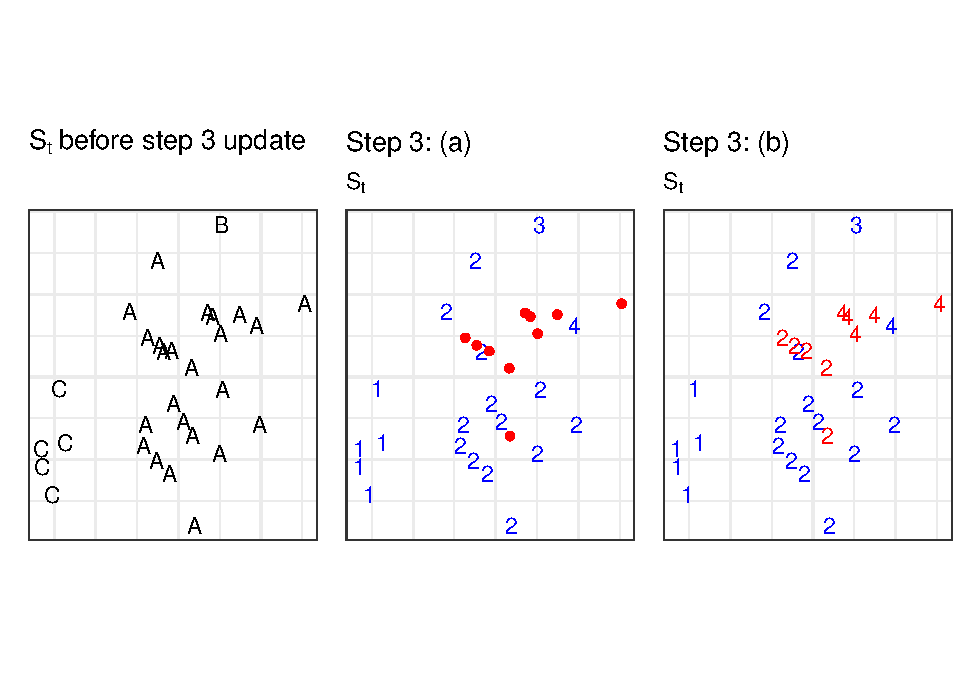
\includegraphics[width=0.8\linewidth]{clustering_paper_files/figure-latex/step3figs-1} 

}

\caption{An example of step 3. In this example, there are 30 hotspots belong to interval $\boldsymbol{S}_t$. (a) 20 out of 30 hotspots belong to both interval $\boldsymbol{S}_t$ and interval $\boldsymbol{S}_{t-1}$. These hotspots succeed their memberships from $\boldsymbol{S}_{t-1}$. They are annotated in blue with membership labels. Points in red are the rest 10 hotspots that only belong to interval $\boldsymbol{S}_t$. (b) For each red point, succeeds the nearest blue label that shares the same component (according to the left plot) with that red point in interval $\boldsymbol{S}_t$. }\label{fig:step3figs}
\end{figure}
\end{Schunk}

\hypertarget{results}{%
\subsubsection{Results}\label{results}}

The result of this spatiotemporal clustering algorithm applied on the
hotspot data is a vector of memberships with length equals to 75936.

\hypertarget{effects-of-parameter-choices}{%
\subsubsection{Effects of parameter
choices}\label{effects-of-parameter-choices}}

There are two parameters that being introduced in the outline of the
algorithm, which are \(AdjDist\) and \(ActiveTime\). The optimal choice
of these two parameters is not known but can be tuned using a
visualization tool.

Considering the relationships between \(AdjDist\), \(ActiveTime\) and
the number of clusters in the clustering result, increase either
\(AdjDist\) or \(ActiveTime\) will usually reduce the number of
clusters. However, if there are large gaps between clusters spatially
and temporally, increase these two parameters will not significantly
reduce the number of clusters. Given one of the metrics to evaluate the
goodness of the clustering result is the gap between clusters, the
optimal choice of \(AdjDist\) and \(ActiveTime\) can be chosen when they
have minimum impact on the number of clusters. However, under this
setting, the optimal \(ActiveTime\) and \(AdjDist\) will approach to
infinitely as the number of clusters approach to 1. Hence, a restriction
needs to be applied on this optimization. Increase of \(ActiveTime\) and
\(AdjDist\) will only be allowed when there is a major fall of the
number of clusters. Based on this rule, a visualization tool inspired by
the scree plot used in the principal component analysis is developed.
Similar to the scree plot, users need to determine the \(ActiveTime\)
and \(AdjDist\) to capture most of the decrease of the number of
clusters. Figure \ref{fig:vis1} and \ref{fig:vis2} show the parameter
tuning process by using this visualization tool. The final choice of
\(ActiveTime\) is \(24\) hours and \(AdjDist\) is \(3000\) metres.

\begin{Schunk}
\begin{figure}

{\centering 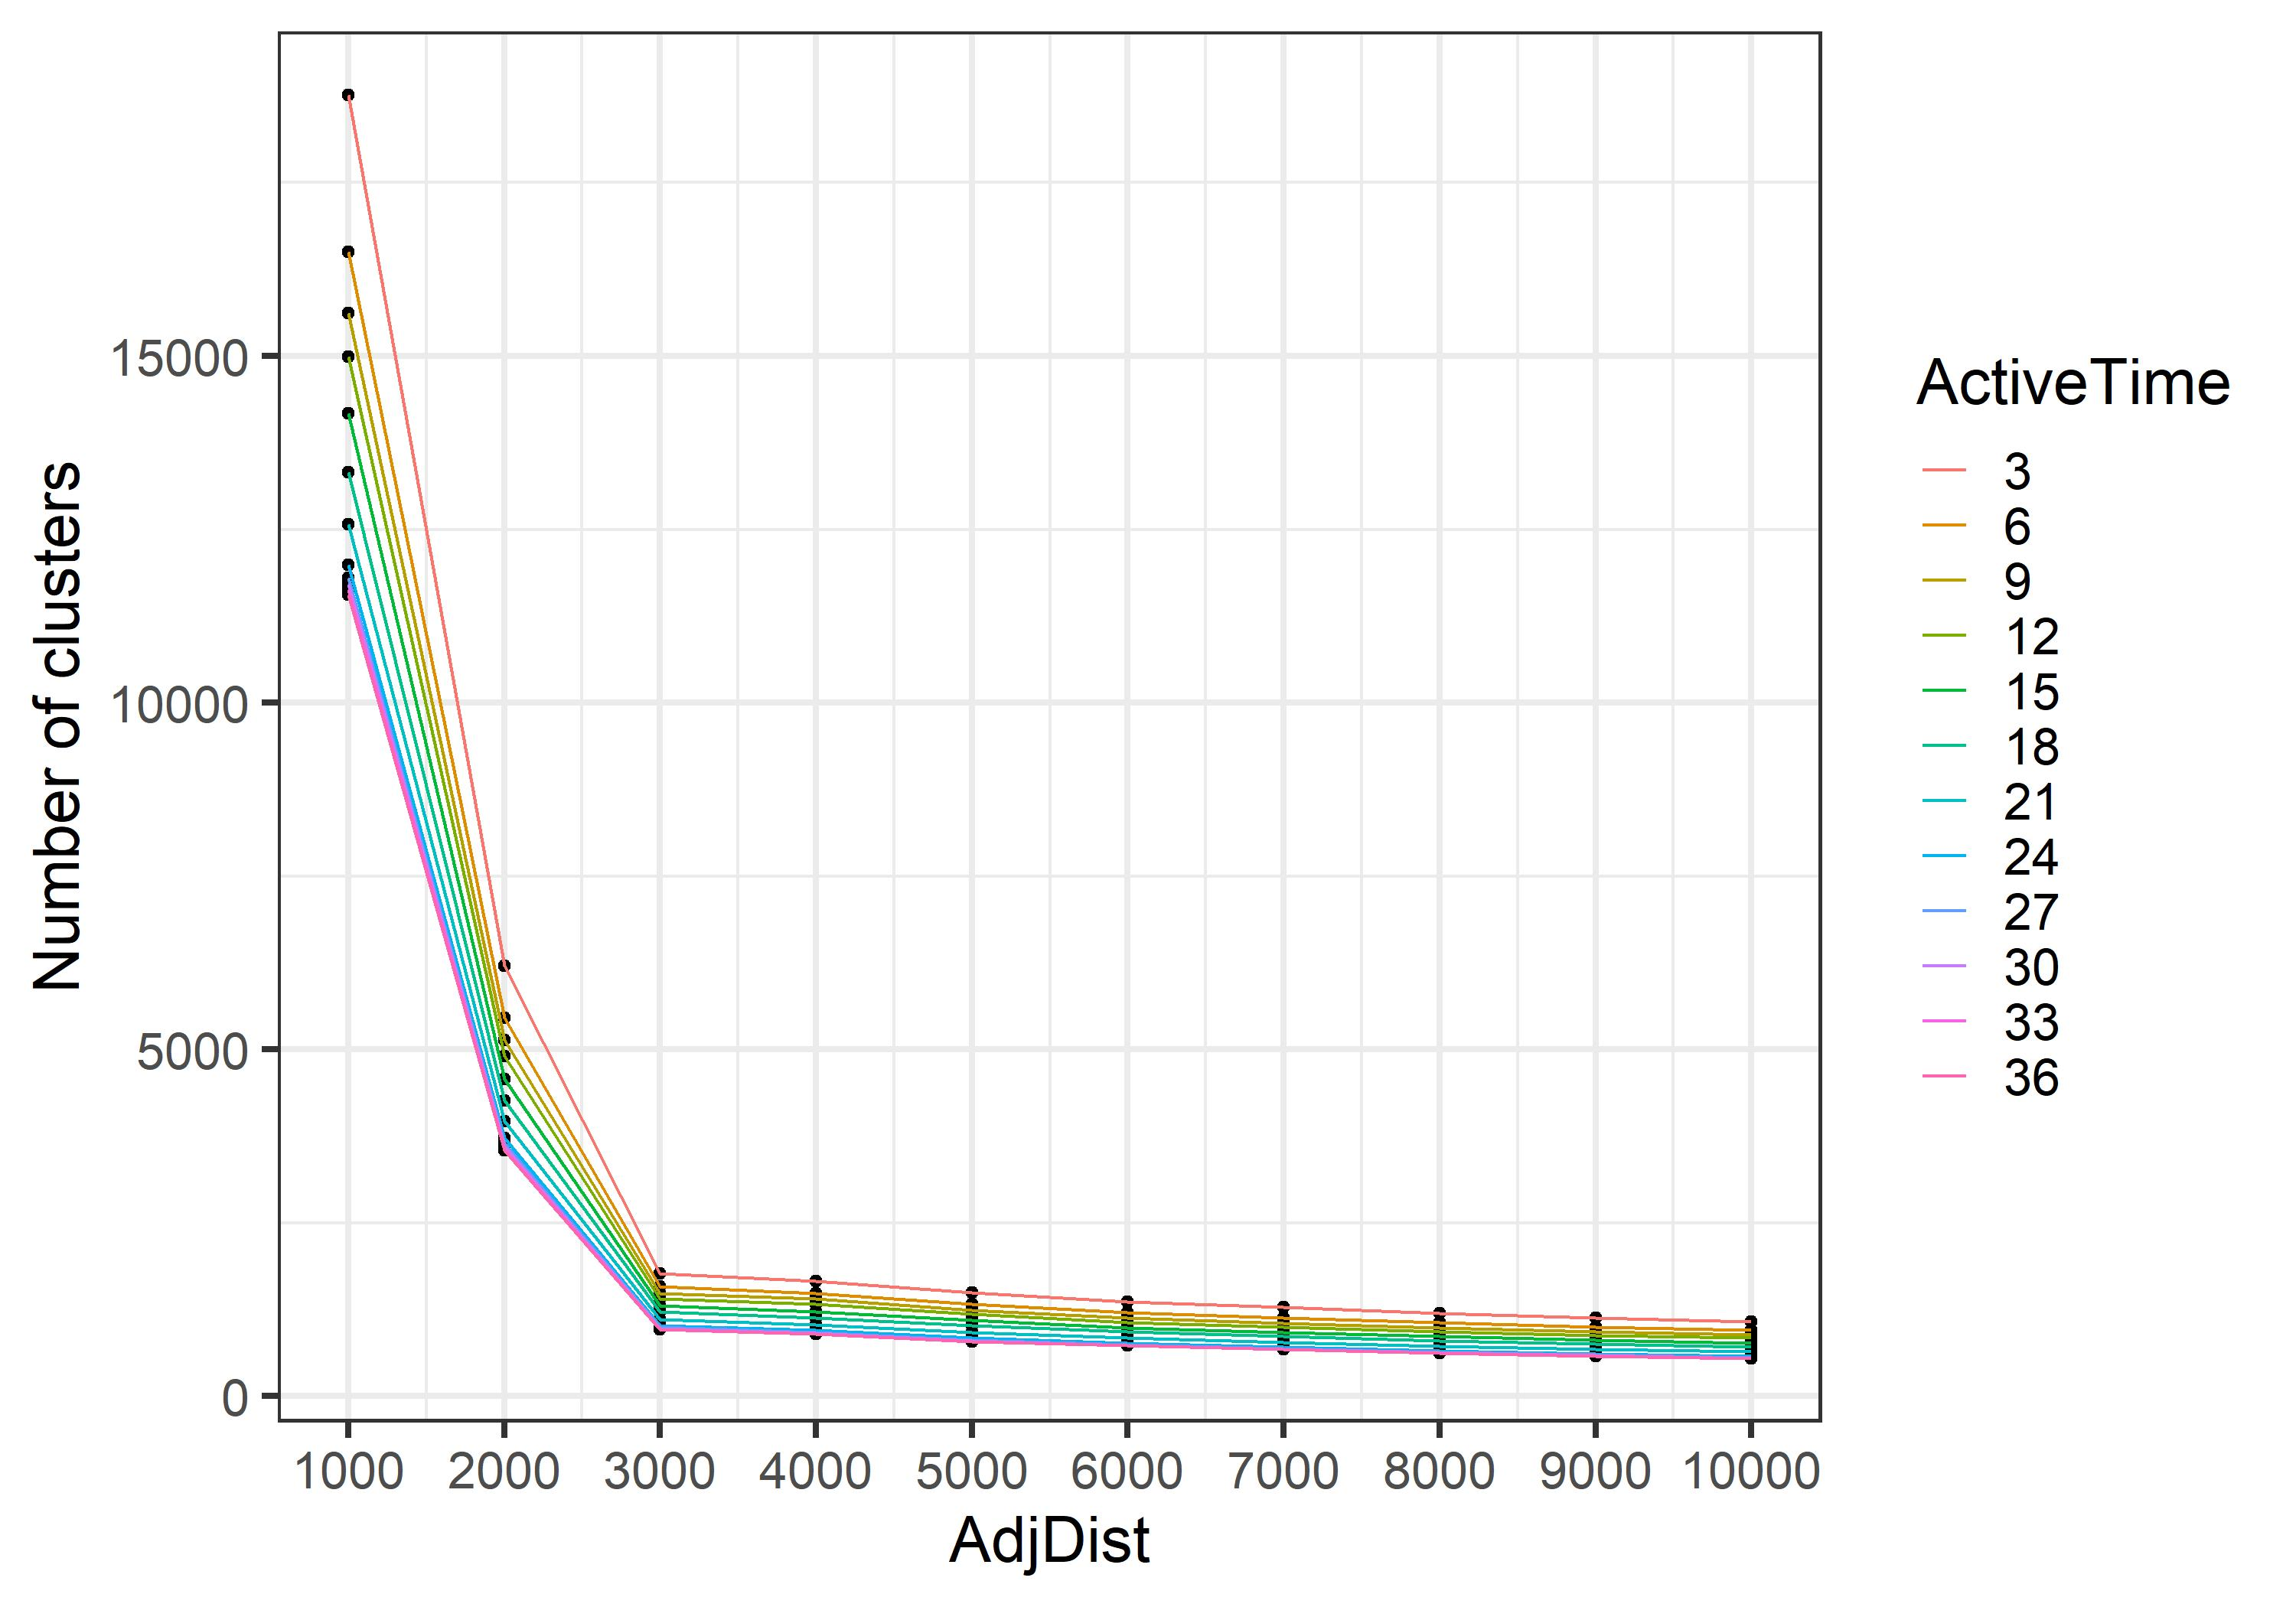
\includegraphics[width=0.8\linewidth]{figures/clustering_tuning_1} 

}

\caption[A visualization tool for parameter tuning ]{A visualization tool for parameter tuning . It works like a scree plot. Major falls of the number of clusters are observed when $AdjDist < 3000$ so the reasonable choice of $AdjDist$ is 3000m.}\label{fig:vis1}
\end{figure}
\end{Schunk}

\begin{Schunk}
\begin{figure}

{\centering 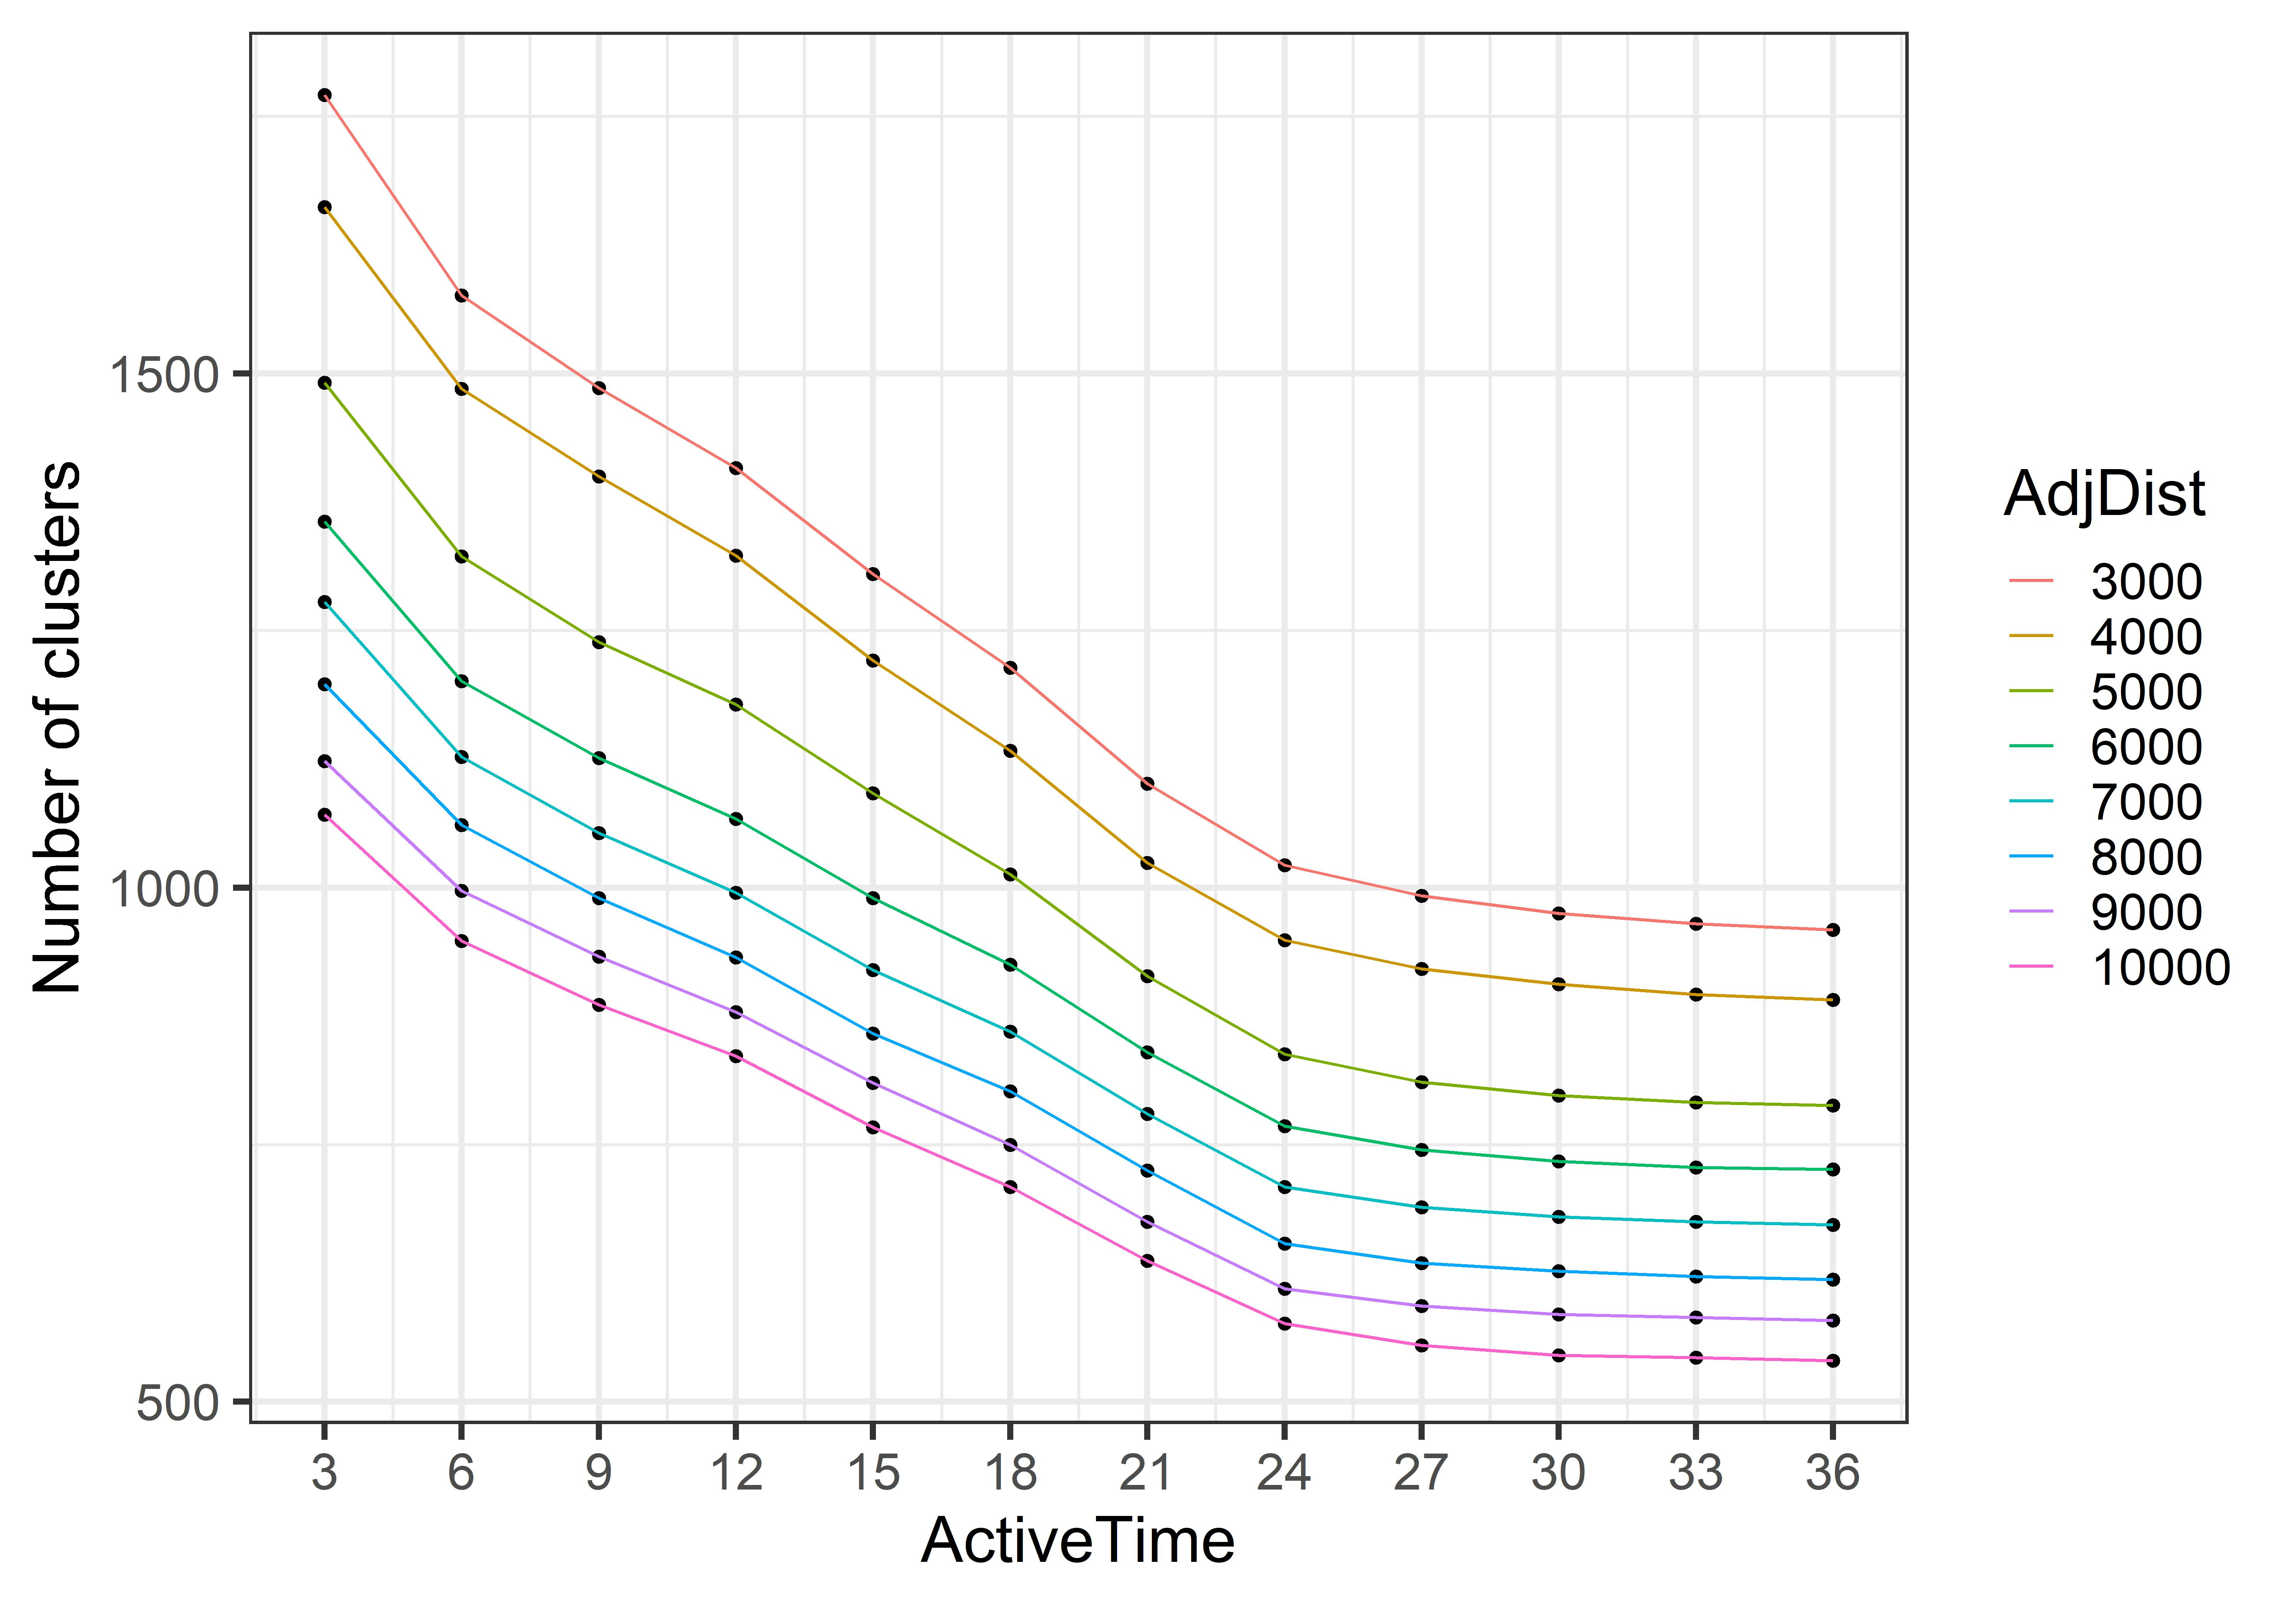
\includegraphics[width=0.8\linewidth]{figures/clustering_tuning_2} 

}

\caption[Major falls of the number of clusteres are observed when $ActiveTime < 24$, so the reasonable choice of $ActiveTime$ is 24 hours]{Major falls of the number of clusteres are observed when $ActiveTime < 24$, so the reasonable choice of $ActiveTime$ is 24 hours.}\label{fig:vis2}
\end{figure}
\end{Schunk}

\hypertarget{application}{%
\subsection{Application}\label{application}}

\hypertarget{determining-the-ignition-point-and-time-for-individual-fires}{%
\subsubsection{Determining the ignition point and time for individual
fires}\label{determining-the-ignition-point-and-time-for-individual-fires}}

Based on the clustering result, ignition location for each cluster can
be computed. The strategy is to select the earliest hotspot of a cluster
as its ignition point. Besides, if there are multiple earliest hotspots
belong to the same cluster, the centroid of these hotspots is used as
the ignition location. According to this method, ignition points over 6
months are given in Figure \ref{fig:clusteringfinalresults} and Figure
\ref{fig:app3}.

\begin{Schunk}
\begin{figure}

{\centering 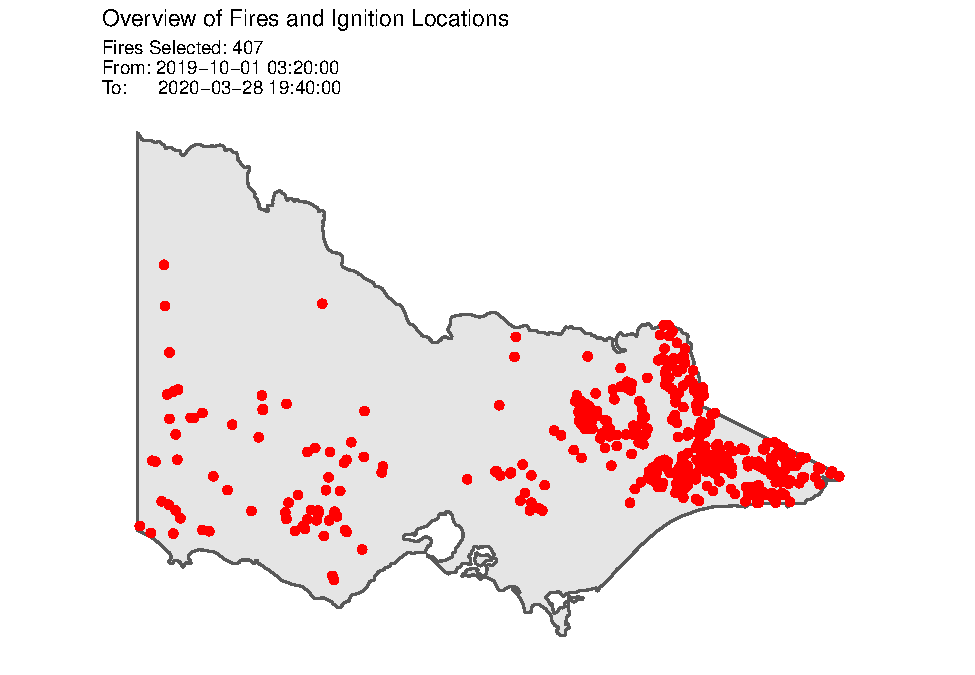
\includegraphics[width=0.8\linewidth]{clustering_paper_files/figure-latex/clusteringfinalresults-1} 

}

\caption[ The distribution of bushfire ignitions in Victoria during 2019-2020 Australian bushfire season]{ The distribution of bushfire ignitions in Victoria during 2019-2020 Australian bushfire season.}\label{fig:clusteringfinalresults}
\end{figure}
\end{Schunk}

\begin{Schunk}
\begin{figure}

{\centering 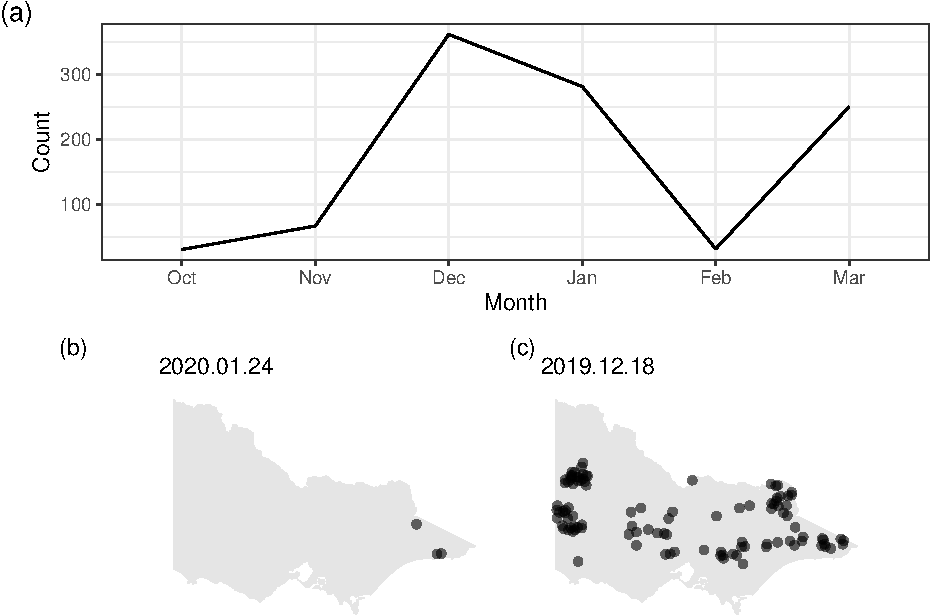
\includegraphics[width=0.8\linewidth]{clustering_paper_files/figure-latex/app3-1} 

}

\caption[(a) Number of bushfires ignited from October 2019 to March 2020]{(a) Number of bushfires ignited from October 2019 to March 2020. (b) The distribution of the bushfire ignitions on a light day (c) and a heavy day. There are 3 ignitions on January 24, 2020 and 106 ignitions on December 18, 2019.}\label{fig:app3}
\end{figure}
\end{Schunk}

\hypertarget{tracking-fire-movement}{%
\subsubsection{Tracking fire movement}\label{tracking-fire-movement}}

Display showing how a fire moves over time, maybe two or more fires

\hypertarget{allocating-resources-for-future-fire-prevention}{%
\subsubsection{Allocating resources for future fire
prevention}\label{allocating-resources-for-future-fire-prevention}}

Merging data with camp sites, CFA, roads, \ldots{}

\hypertarget{implementation}{%
\subsection{Implementation}\label{implementation}}

The algorithm is available in the R package \pkg{spotoroo}.

\hypertarget{installation}{%
\subsubsection{Installation}\label{installation}}

The package can be installed from CRAN using

\begin{verbatim}
install.packages("spotoroo")
\end{verbatim}

and the developmental version from github using

\begin{verbatim}
install.packages("remotes")
remotes::install_github("TengMCing/spotoroo")
\end{verbatim}

\hypertarget{usage}{%
\subsubsection{Usage}\label{usage}}

A sample data set is provided with the package, to illustrate its use.
The function \texttt{hotspot\_cluster} performs the spatial clustering.
Here we have called it fir the sample data, specifying the spatial and
temporal variables (lon, lat, obsTime), and several parameters to the
algorithm. A summary of the results is printed when the algorithm
completes.

\begin{Schunk}
\begin{Sinput}
library(spotoroo)
library(tidyverse)
result <- hotspot_cluster(hotspots,
                          lon = "lon",
                          lat = "lat",
                          obsTime = "obsTime",
                          activeTime = 24,
                          adjDist = 3000,
                          minPts = 4,
                          minTime = 3,
                          ignitionCenter = "mean",
                          timeUnit = "h",
                          timeStep = 1)
\end{Sinput}
\begin{Soutput}
#> 
\end{Soutput}
\begin{Soutput}
#> -------------------------------- SPOTOROO 0.1.0 --------------------------------
\end{Soutput}
\begin{Soutput}
#> 
\end{Soutput}
\begin{Soutput}
#> -- Calling Core Function : `hotspot_cluster()` --
\end{Soutput}
\begin{Soutput}
#> 
\end{Soutput}
\begin{Soutput}
#> -- 1 time index = 1 hours
\end{Soutput}
\begin{Soutput}
#> v Transform observed time > time indexes
\end{Soutput}
\begin{Soutput}
#> i 970 time indexes found
\end{Soutput}
\begin{Soutput}
#> 
\end{Soutput}
\begin{Soutput}
#> -- activeTime = 24 time indexes | adjDist = 3000 meters
\end{Soutput}
\begin{Soutput}
#> v Cluster
\end{Soutput}
\begin{Soutput}
#> i 16 clusters found (including noise)
\end{Soutput}
\begin{Soutput}
#> 
\end{Soutput}
\begin{Soutput}
#> -- minPts = 4 hot spots | minTime = 3 time indexes
\end{Soutput}
\begin{Soutput}
#> v Handle noise
\end{Soutput}
\begin{Soutput}
#> i 6 clusters left
\end{Soutput}
\begin{Soutput}
#> i noise proportion : 0.935 %
\end{Soutput}
\begin{Soutput}
#> 
\end{Soutput}
\begin{Soutput}
#> -- ignitionCenter = 'mean'
\end{Soutput}
\begin{Soutput}
#> v Compute ignition points for clusters
\end{Soutput}
\begin{Soutput}
#> i average hot spots : 176.7
\end{Soutput}
\begin{Soutput}
#> i average duration : 131.9 hours
\end{Soutput}
\begin{Soutput}
#> 
\end{Soutput}
\begin{Soutput}
#> -- Time taken = 0 mins 2 secs for 1070 hot spots
\end{Soutput}
\begin{Soutput}
#> i 0.002 secs per hot spot
\end{Soutput}
\begin{Soutput}
#> 
\end{Soutput}
\begin{Soutput}
#> --------------------------------------------------------------------------------
\end{Soutput}
\end{Schunk}

For this sample of data, the result contains `r length(unique(result\$))

\begin{Schunk}
\begin{figure}

{\centering 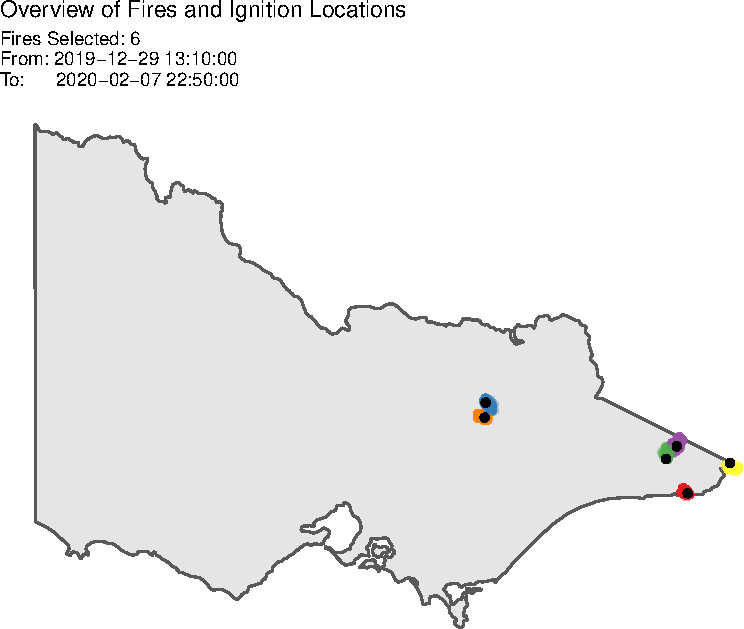
\includegraphics[width=0.8\linewidth]{clustering_paper_files/figure-latex/unnamed-chunk-8-1} 

}

\caption[Automatic plot of results]{Automatic plot of results}\label{fig:unnamed-chunk-8}
\end{figure}
\end{Schunk}

\begin{Schunk}


\begin{center}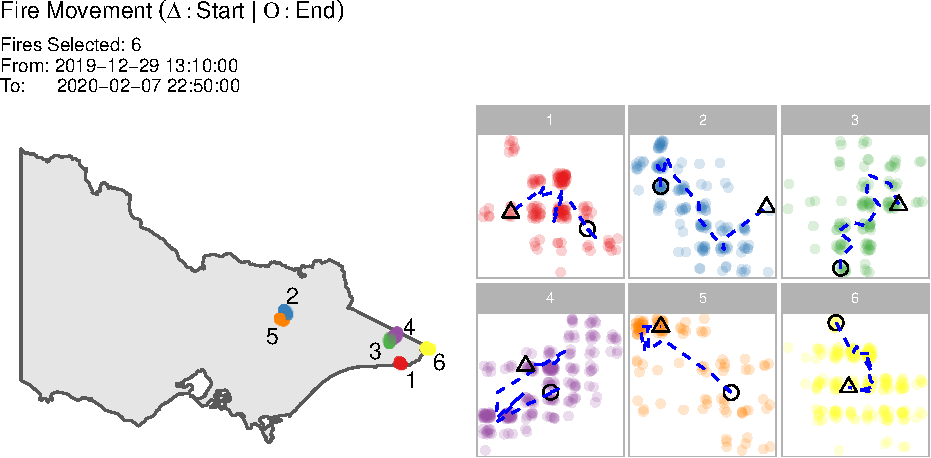
\includegraphics[width=1\linewidth]{clustering_paper_files/figure-latex/unnamed-chunk-9-1} \end{center}

\end{Schunk}

\begin{Schunk}


\begin{center}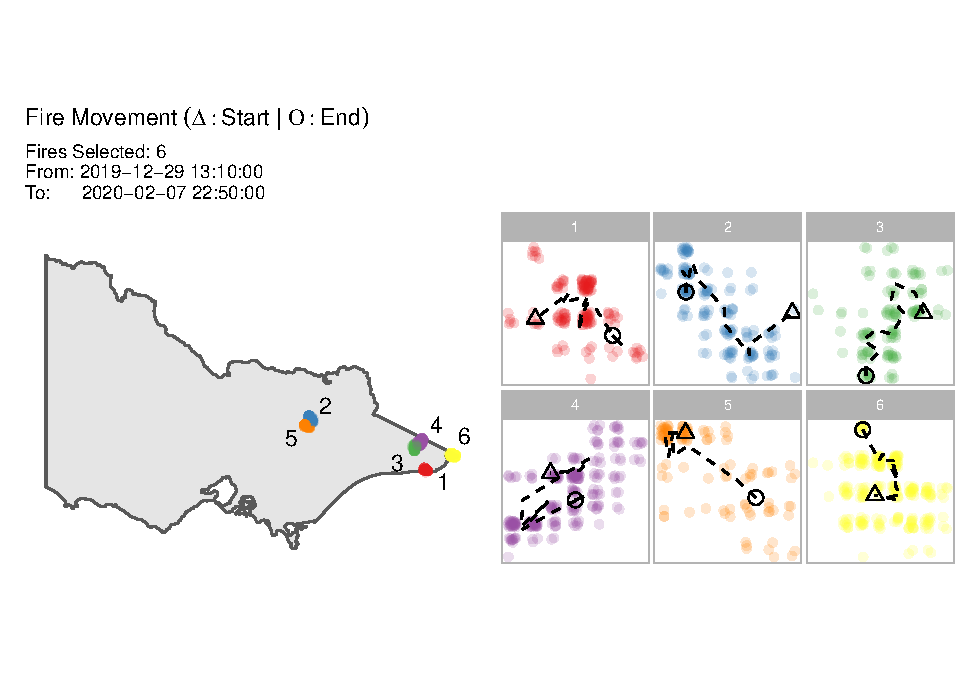
\includegraphics[width=1\linewidth]{clustering_paper_files/figure-latex/unnamed-chunk-10-1} \end{center}

\end{Schunk}

\hypertarget{functions}{%
\subsubsection{Functions}\label{functions}}

\hypertarget{summary}{%
\subsection{Summary}\label{summary}}

\hypertarget{acknowledgements}{%
\subsection{Acknowledgements}\label{acknowledgements}}

\begin{itemize}
\tightlist
\item
  The code and files to reproduce this work are at XXX
\item
  Data on hotspots can be downloaded from XXX
\end{itemize}

\bibliography{RJreferences}


\address{%
Weihao Li\\
Monash University\\%
Econometrics and Business Statistics\\
%
%
%
\\\href{mailto:wlii0039@student.monash.edu}{\nolinkurl{wlii0039@student.monash.edu}}
}

\address{%
Emily Dodwell\\
??\\%
line 1\\ line 2\\
%
%
%
\\\href{mailto:emdodwell@gmail.com}{\nolinkurl{emdodwell@gmail.com}}
}

\address{%
Dianne Cook\\
Monash University\\%
Econometrics and Business Statistics\\
%
%
%
\\\href{mailto:dicook@monash.edu}{\nolinkurl{dicook@monash.edu}}
}
